\documentclass{article}
\usepackage{graphicx}
\usepackage{multirow}
\usepackage{geometry}
\usepackage{titlesec}

\usepackage{enumerate}

\geometry{top=1.3in, bottom=1.3in, left=1.2in, right=1.2in}
\setcounter{secnumdepth}{4}

\titleformat{\paragraph}
{\normalfont\normalsize\bfseries}{\theparagraph}{1em}{}
\titlespacing*{\paragraph}
{0pt}{3.25ex plus 1ex minus .2ex}{1.5ex plus .2ex}

\begin{document}

%page 1
\vspace*{3em}
\begin{center}
{\rule{11cm}{0.01cm} \\ \tiny~
\\ \large \sc{UM--SJTU ~Joint Institute \\ \tiny ~
\\ \large Introduction to Engineering \\ \tiny ~ 
\\ \large VG100 \\ \tiny ~}
\rule{11cm}{0.01cm}  
\vspace*{3.5em}
\\  \large\sc{Final Report on Project 2 \\ \tiny ~ \\ \huge Motion Tuner\\ ~ \\ \Large Group 3 Trinity}}
\end{center}

\normalsize
\vspace*{10em}
\begin{center}
\begin{tabular}{cl}
\large
\vspace{0.3em} Xie Shuxiang&516370910070\vspace{0.3em}\\ 
\large
Ma Kerui\vspace{0.3em} &516370910106 \vspace{0.3em}\\ 
\large
Wang Ren\vspace{0.3em} &516370910177 \vspace{0.3em}\\ 
\large
Zhu Boying\vspace{0.3em} &516370910165 \vspace{0.3em}\\ 
\large
Guo Chengzhang\vspace{0.3em} &516021910639 \vspace{0.3em}\\ 
 
\end{tabular}
\end{center}

\normalsize
\vspace*{1em}
\begin{center}
\large
$\hspace{1em}Instructor$\\
\vspace*{1em}
\begin{tabular}{lcl}
\large
Professor\hspace{0.5em}\vspace{0.3em} &\hspace{0.5em}Yanfeng Shen\hspace{0.5em}&\hspace{0.5em}Ph.D\\ 
Professor\hspace{0.5em} &\hspace{0.5em}Cynthia Vagnetti \hspace{0.5em}&\hspace{0.5em}Ph.D\\ 
\end{tabular}
\end{center}


%page1.5 mulu
\newpage
\tableofcontents


%%%%%%%%
%\newpage
\section{Executive Summary}


%%%%%%
%\newpage
\section{Acknowledgement}


%%%%%
%\newpage
\section{Introduction}

%%%%%%
%\newpage
\section{Problem}
\subsection{Statement of the problem}
\hspace*{2em}Many citizens find themselves under the pressure over moderate and too busy to pursue for happiness. They are in unhealthy mental conditions but lack for convenient ways to get happiness. People have tried to get happiness since the happiness lesson in Haward, aiming to teach people to be happy, has become one of the most popular courses. According to China Daily, many high school students find themselves under high pressure. Even though they want to do some exercise sometimes, the space is limited.\\
\hspace*{2em}We choose dance to help people relax because it is convenient and low cost. Compared to other healthy relaxing ways like jogging and walking, dancing can be indoors, not influenced by the weather or the air pollution. The cost for dance is quite low. Traditional dancing machines takes too much space and not suitable for work places and study rooms. What?s more, this kind of machines is unfriendly for dancing beginners.\\
�\hspace*{2em}As a result, traditional dancing machine cannot provide users with anytime and anywhere dance. \\
\subsection{Summary of the problem}
\hspace*{2em}In summary, people need ways to relax because they are busy and under pressure. Dance can help people to get happiness, but traditional dancing machine exists these problems:
\begin{enumerate}[\hspace*{3em}(1)  ]
\item Too much space
\item Unavailable in most places
\item Difficult for beginners
\end{enumerate}

%%%%%%%
\section{Need and Validation}
\subsection{Needs}
\hspace*{2em}Our product is to provide people with convenient ways to get happiness.
\hspace*{2em}To make our product convenient, the device should meet the needs of:
\begin{enumerate}[\hspace*{3em}(1)]
\item Portable: The device should be able to be carried anywhere, like an App or a bracelet
\item Low cost: The price should not be a burden for most people
\item Multi-function: There should be more than one kinds of motion detected and more than one types of music produced.
\end{enumerate}
\hspace*{2em}There are also some constrains:
\begin{enumerate}[\hspace*{3em}(1)]
\item Database: To make different functions, we need to build a large database to analyze, which may be too large for an iphone.
\item Budget: Smaller the chip, higher the price.
\end{enumerate}
\subsection{Validation}
\hspace*{2em}Our device can meet with the criteria:
\begin{enumerate}[\hspace*{3em}(1)]
\item For portable, our chip is only 1mm*1.5mm, which can be put into a bracelet.
\item For affordable, our device is only 130 RMB, which is only one thirds of the prices of dancing machines and one tenths of the prices of motion detectors in the market.  So, it will be affordable for most people. 
\item For multi-function, our chip will transmit 9 groups of acceleration per second, quickly enough for detecting motions and creating music. We also simplify 9 numbers to 1 to save space.
\end{enumerate}

%%%%%%
\section{Solution}

\subsection{Mobile Terminal Part}

\subsubsection{Flow Chart}

   First the motion of one person is detected by the sensor and become raw data.
   Then the raw data is filtered into acceleration data. 

   The filter mainly did two things.
   One is to abandon the useless data such as temperature and the other is to
   map the acceleration data into float point value between 0 to 5. 

   After that, the acceleration data will be processed through one of the
   following function, which are the \textbf{Matcher} and the \textbf{Scaler}. 

   After the the process of \textbf{Matcher} or \textbf{Scaler} function, one
   sound track is created and finally the multiple sound tracks are mixed into
   the final audio. 

\subsubsection{Index Script}

The Unity Engine first recognize the index script and hand over its control to
it.  
Thus, we use the index script to get access to the 
\textbf{gyroscope}, \textbf{speaker} of the mobile phone, 
 ask for \textbf{memory}, create \textbf{main loop} (the loop in which the
 program will be in after initial setup), and call for 
\textbf{Matcher} and \textbf{Scaler} functions. 
The flow chart of the index script is shown in Figure~\ref{indexScript}.


\begin{figure}[H]

\begin{minipage}[b]{0.5\linewidth}
\centering
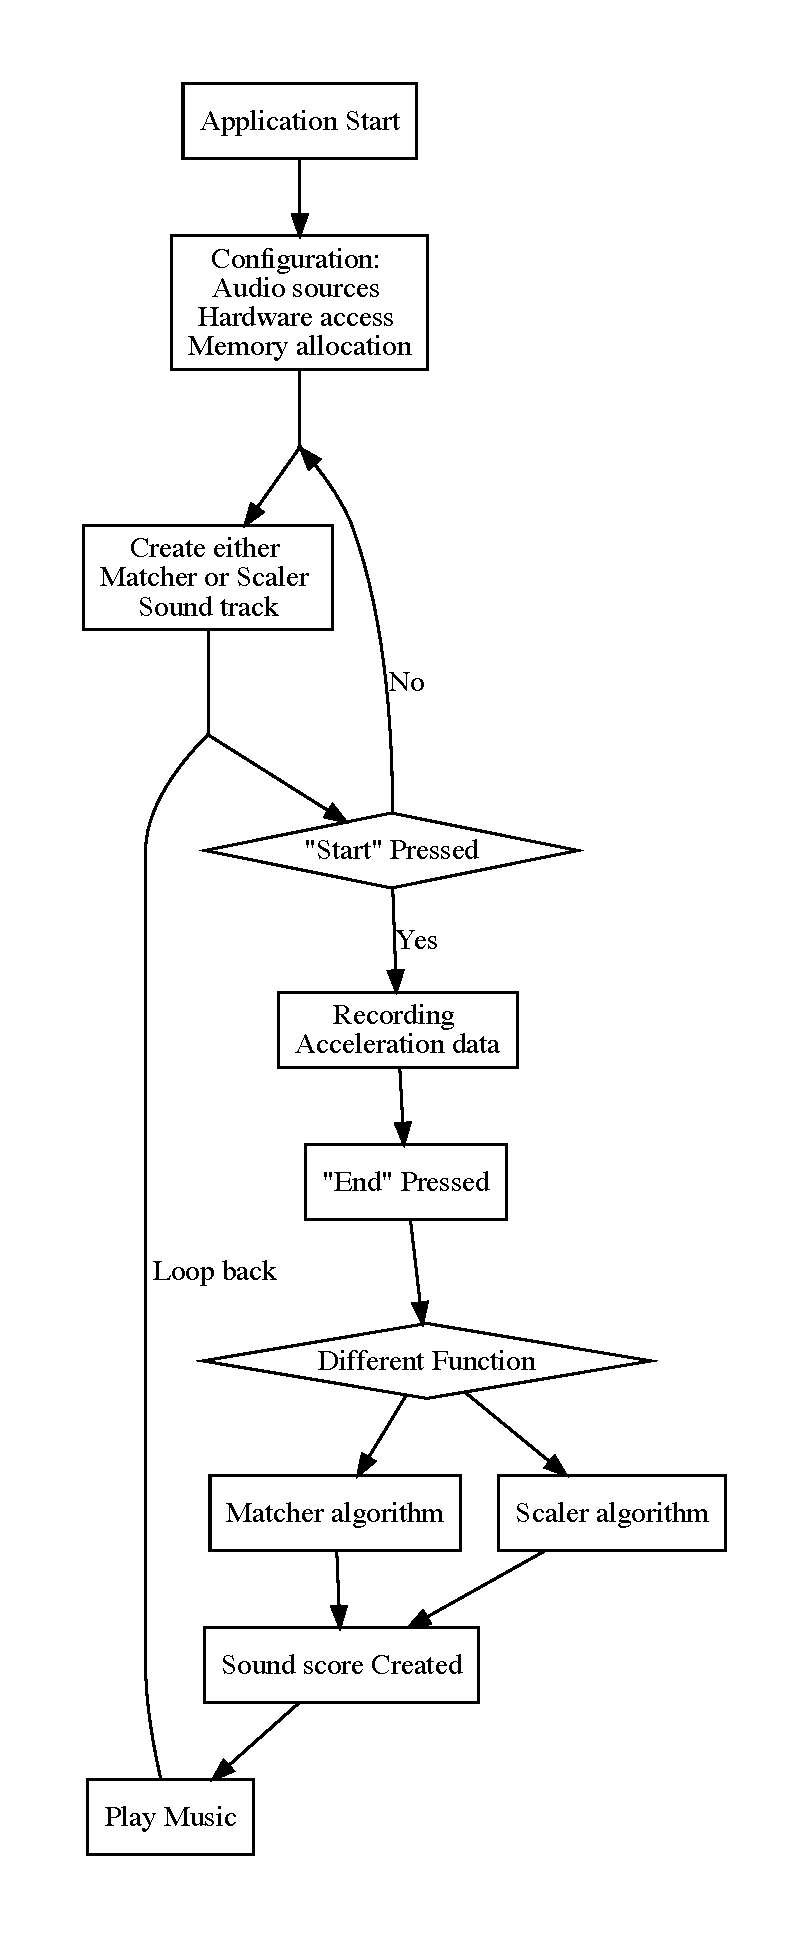
\includegraphics[height=0.95\textheight]{figWR/a}
\caption{Flow Chart of the Index Script}
\label{indexScript}
\end{minipage}%%
%
\begin{minipage}[b]{0.5\linewidth}
\centering
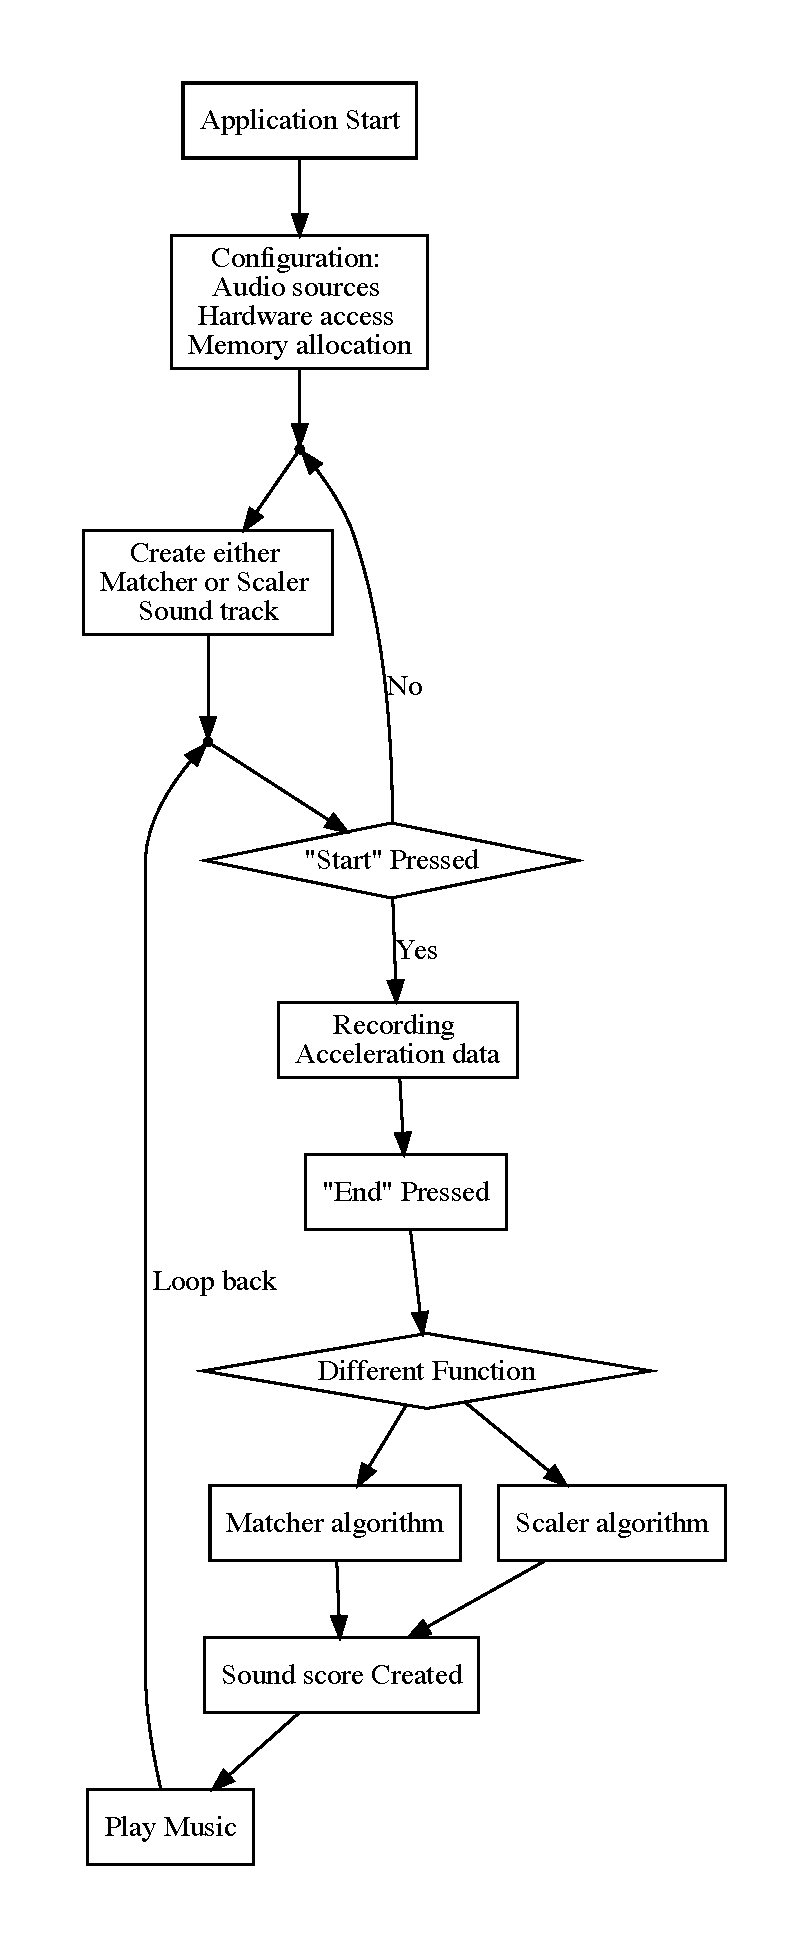
\includegraphics[width=1\linewidth]{figWR/ma}
\caption{Flow Chart of Matcher}
\label{FlowMatcher}
\vspace{4ex}
\centering
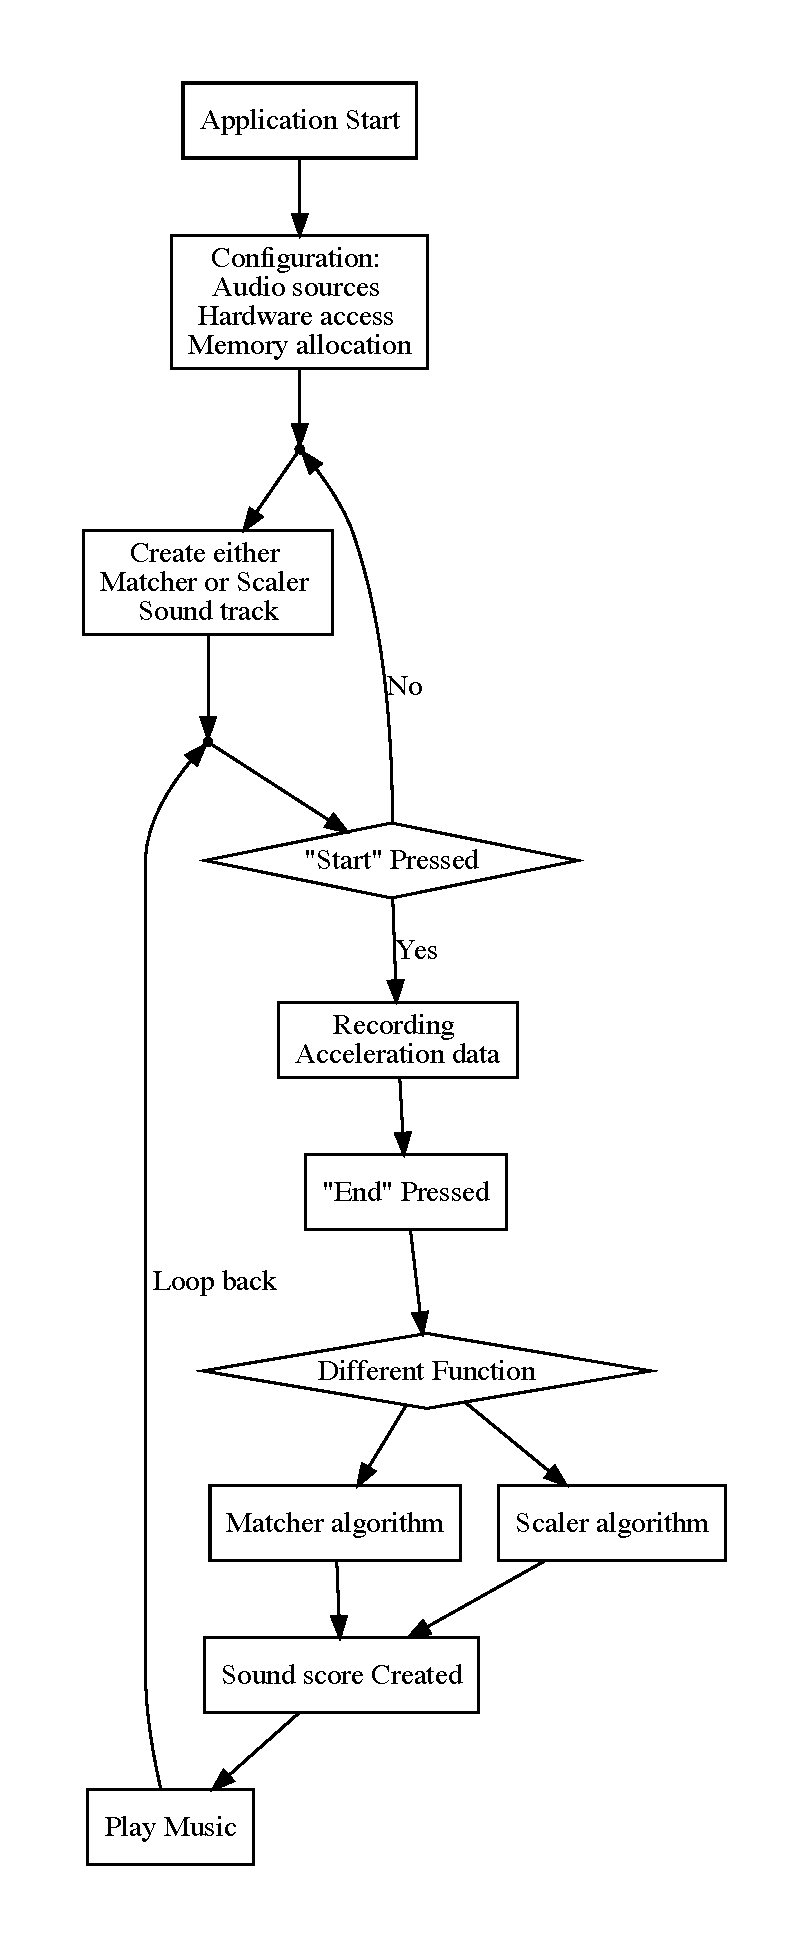
\includegraphics[width=1\linewidth]{figWR/sc}
\caption{Flow Chart of Scaler}
\label{FlowMatcher}
\vspace{4ex}
\end{minipage}%%
\end{figure}

\subsubsection{Scaler algorithm}

For the \textbf{Scaler} part, also suppose we have the acceleration data. Then
we separate them into 10 time intervals equally. And we find the max value in
each interval. Then the ruler is created based on the max value and the min
value of the acceleration data. The ruler create 7 blanks vertically for there
is 7 tones in one music period, which are ``do re mi fa so la ti''. Fill in the
blank and finally a music score is created and it produces one sound track. 

The visual of the \textbf{Scaler} process is shown by step in
Figure~\ref{scalerStep0} to Figure~\ref{scalerStep2}. 

\begin{figure}[H]
\centering
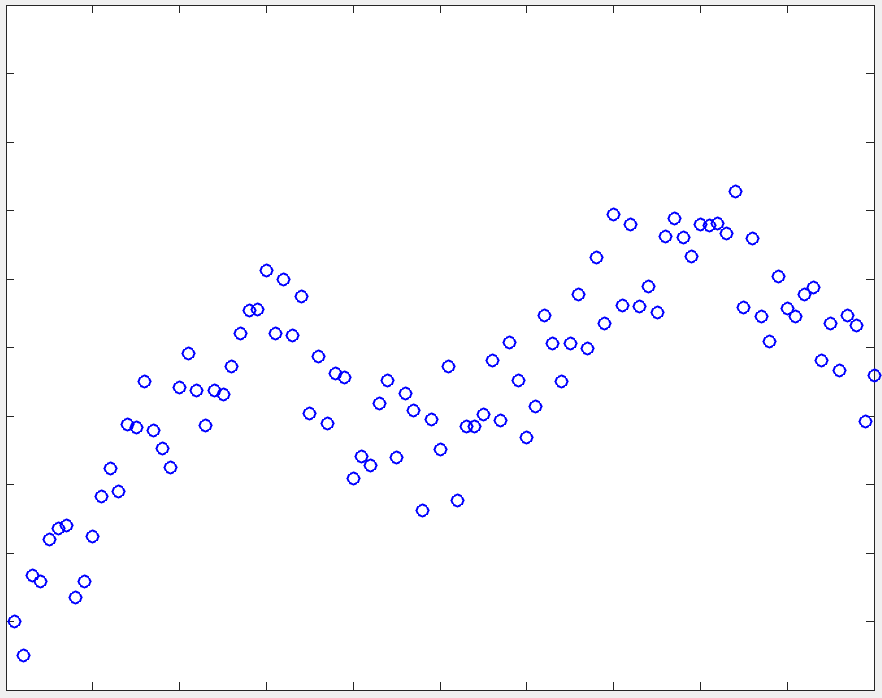
\includegraphics[width=0.35\linewidth]{figWR/scaler0}
\caption{Scaler Process, original data}
\label{scalerStep0}
\end{figure}


\begin{figure}[H]
\centering
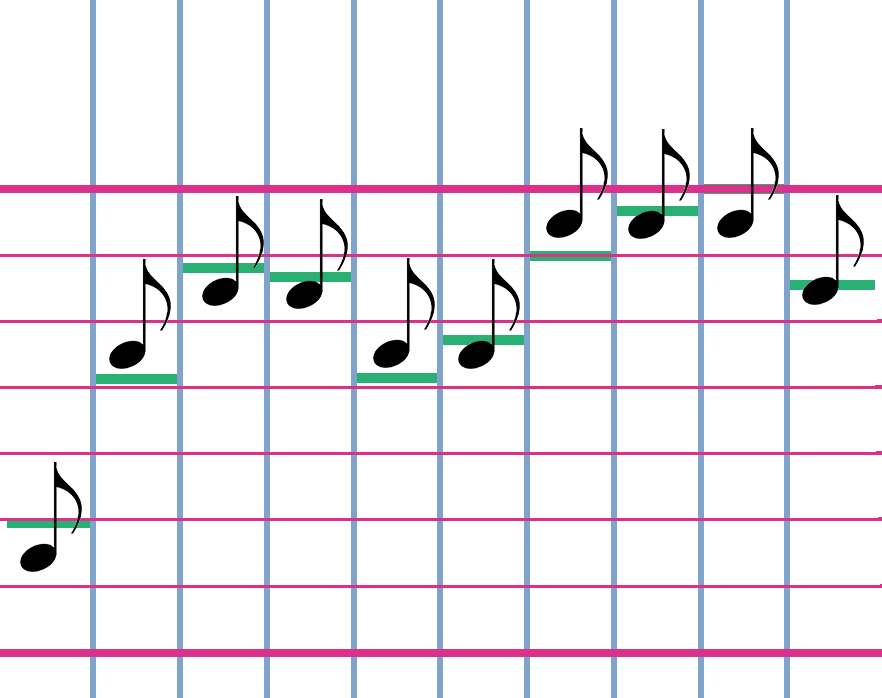
\includegraphics[width=0.35\linewidth]{figWR/scaler1}
\caption{Scaler Process, split and create ruler}
\label{scalerStep1}
\end{figure}


\begin{figure}[H]
\centering
\newcommand{\widthOfScalerStepFigure}{5cm}
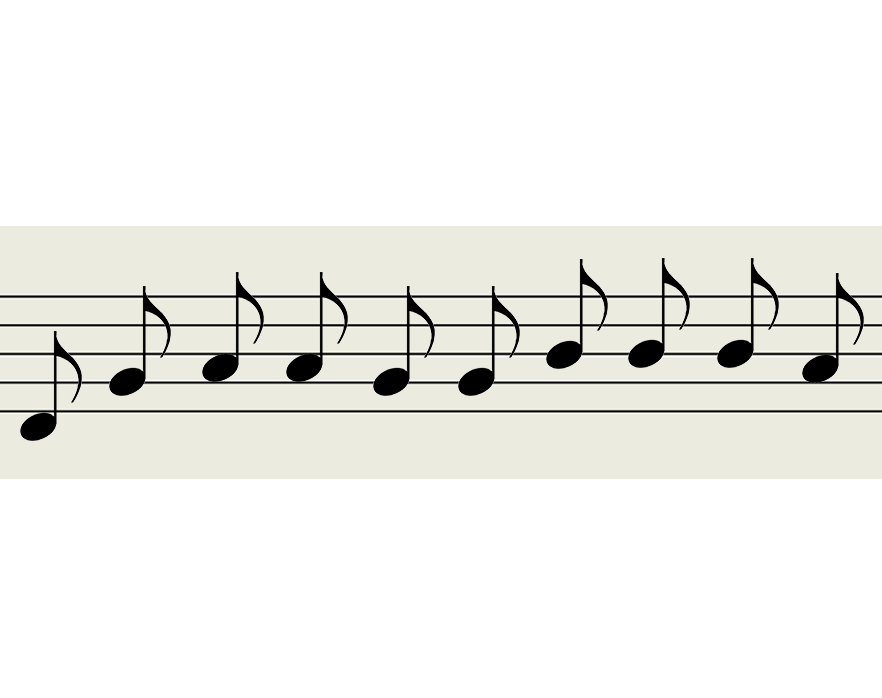
\includegraphics[width=0.35\linewidth]{figWR/scaler2}
\caption{Scaler Process, final music score}
\label{scalerStep2}
\end{figure}


\subsubsection{Matcher algorithm}

For the \textbf{Matcher} part, suppose we have the acceleration data, then we
compared it with three pre-configured answers, calculate the difference between
answers and real data. The one that has the least sum of absolute value is the
audio clip we select. Then the corresponding sound track is created. 

The visual of the \textbf{Matcher} process is shown in Figure~\ref{matcherStep0}
and Figure~\ref{matcherStep1}.


\newcommand{\widthOfMatcherFigure}{9cm}

\begin{figure}[H]
\centering
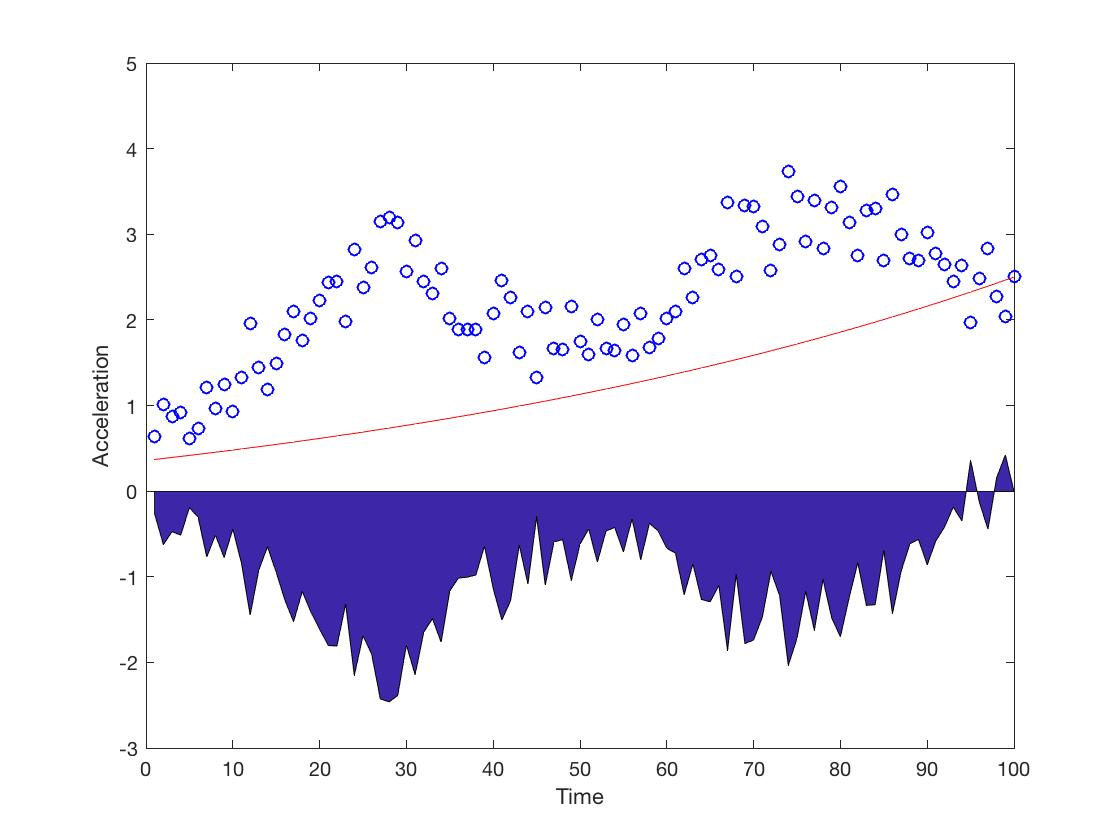
\includegraphics[width=\widthOfMatcherFigure]{figWR/matcher1}
\caption{Matcher Process, Wrong music}
\label{matcherStep0}
\end{figure}

\begin{figure}[H]
\centering
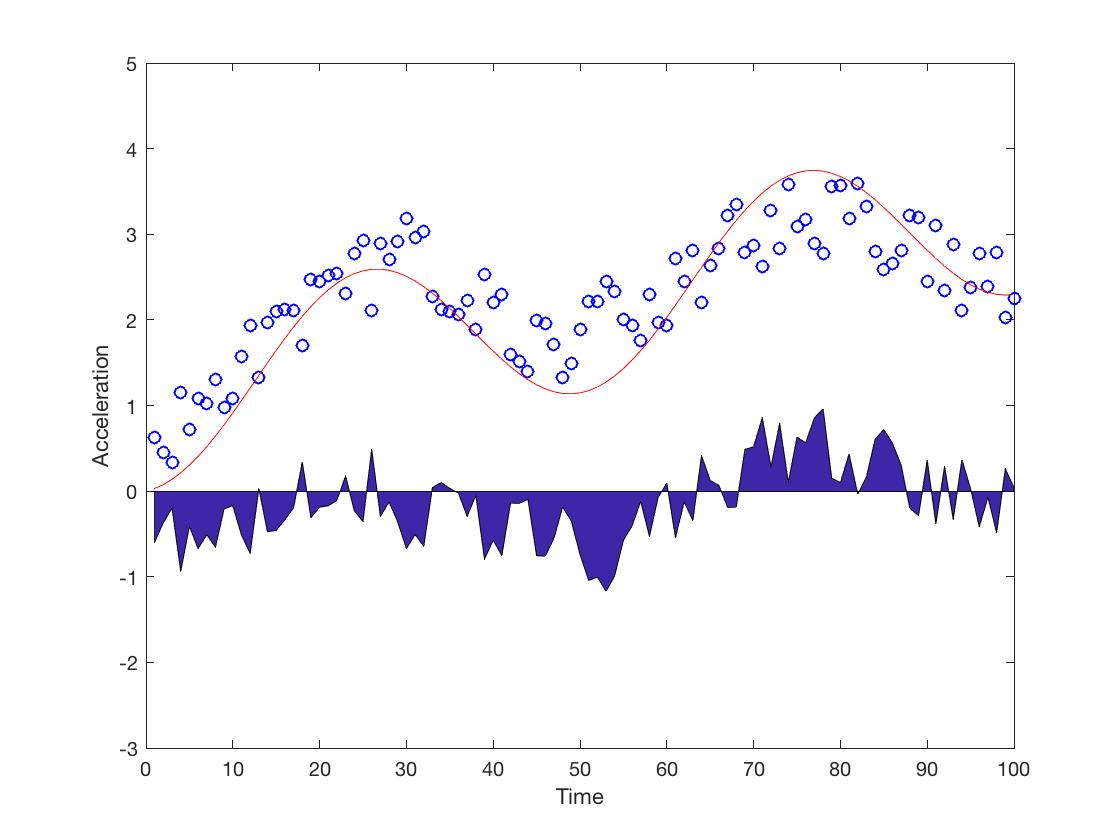
\includegraphics[width=\widthOfMatcherFigure]{figWR/matcher2}
\caption{Matcher Process, Right music}
\label{matcherStep1}
\end{figure}

\subsubsection{Mixer}

After we have multiple sound tracks through either of the previous process, we
mix them together and create the final audio. Feel free to play it. 

\subsection{PC Terminal}

Besides the cellphone terminal part, we also designed a PC terminal part,
because when users dance, cellphones in hands are not safe enough. Cellphones
might be thrown out and hurt someone and then be broken. Moreover, the
cellphones are too heavy to carry when doing some fierce action. So developing a
safer and lighter bracelet is necessary. The second part of our product can
exactly satisfy the needs. 

The second part consists of a bracelet and a PC terminal. The bracelet contains
the sensor JY901, the bluetooth module and batteries. More specifically, the
sensor JY901 can detect data, the bluetooth module can transfer data to the
terminal and the batteries can power both JY901 and bluetooth. Overall, the
bracelet mainly does the detecting job. On the other hand, the PC terminal
mainly does the analyzing and generating jobs. The software on PC terminal
developed by Unity3D can apply several different algorithm to analyze the data,
so that the origin motion kind of the users can be defined. Then by comparing
different conditions prepared previously, the software can mix and play all
kinds audio source. 


\subsubsection{Hardware}
\paragraph{Attitude Sensor JY901}

The sensor JY901 is a attitude sensor that can detect the
acceleration, the angle of avertence and angular velocity. The sensor itself
consists of three-axis gyroscope, three-axis acceleration sensors, three-axis
digital compass and some other motion sensors. The sensor JY901 has the
following characteristics: 


\begin{figure}[H]
\centering
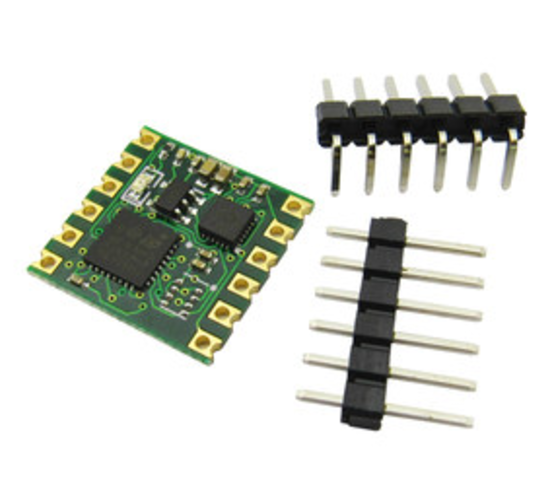
\includegraphics[width=0.4\textwidth]{Pics/imu}
\caption{JY901 Sensor}
\label{matcherStep1}
\end{figure}

\begin{itemize}
\item Flexible data outputting ports. (I2C, SPI, TTL are supported)
\item High speed data outputting rate. (Highest 500Hz)
\item Low power consumption. (17mA)
\item Short and stable initializing time. 
\item Support software development. 
\end{itemize}
\paragraph{Bluetooth Module}

It is connected with the JY901 sensor used for data transmission. In the serial
protocol, the bluetooth plays a role of an imaginary COM port whose name is
“COM6” on the Windows platform. 


\paragraph{Battery}

We use two chargeable batteries to power both JY901 sensor and the bluetooth
module. Each battery’s size is about 1cm*2cm*0.3cm which is very small. However,
each battery can provide 3.3V voltage and about 200 mAh electric charge. Since
the consumption of sensor JY901 is very small, the battery’s life is able to
ensure the normal work of our product. 


\paragraph{Fabrication}

We totally use two 3.3 V batteries to power both the bluetooth module and the
sensor. The reason why we don’t use one battery to power the device is that the
voltage is too small and can not last long. The assembling detail is that, the
positive side connects with the VCC port and the negative side connects with GND
port. The communication between the sensor and the bluetooth is realized by the
connection of RX ports and TX ports.  

\subsubsection{Software}
\paragraph{Data collection algorithm (same with the Mobile terminal part)}
\paragraph{Data transmission algorithm}

Programming Language: C\#

Input: All kinds of data collected by the sensor JY901, including acceleration,
angular acceleration, temperature and so on in 16 hexadecimal.   

Output: Acceleration readings of three axises in 10 hexadecimal. 

Algorithm: The algorithm includes mainly two functions which are''
``ReceiveData()'' and'' ``ReadData()'' and they each has their own thread. In
the initialization part “void Update()” function, we create and open two threads
one by one which can ensure that the data path is clear and efficient. 

Then in function ``ReceiveData()'', an empty string and a buffer byte are
created to store and transport the data collected. Since the “55” in 16
hexadecimal equals to “85” in 10 hexadecimal and all the data we need starts
with “55” in 16 hexadecimal, the “if” sentences are applied. After all the
suitable data have been collected, we add the string to the queue created as a
data pool using the order “queueDataPool.Enqueue(string)”. 

In function ``ReadData()'', we first use the thread different from the previous
one. All the data source in the part are from the queue acting as data pool.
Here another buffer is created to store the data read out of the queue. We read
data out one by one, when the length of the buffer reaches 22 which is the
length we need, the buffer will be stored as formal data and then be cleared.
Please note that since in the “ReceiveData” part we already judge what kind of
data to collect, in the queue the data should starts with “85” in 10 hexadecimal
and we don’t need to set conditions again. Then there is the calculation part,
take the data starts with “5551” in 16 hexadecimal as example. After “5551” the
three axises accelerations are stored in two digits. The data format of the
queue is “string”, so we need to transform data which is “string in 16
hexadecimal” to “int in 10 hexadecimal”. The function
“Int16.Parse(stroutpool[4].ToString(),System.Globalization.NumberStyles.AllowHexSpecifier)” 
is applied. Thus we can calculate the accelerations out one by one.

\paragraph{Data analysis algorithm (same with the Mobile terminal part)}

\paragraph{Audio source generating algorithm (same with the Mobile terminal
  part)} 

%\subsubsection{Working Principles}

%%%%%%%%%%
%\newpage
\section{Objectives}
\subsection{Difficulties}
\hspace*{2em}Since we divided Part 4\&5 into two parts, the mobile terminal part
and the PC terminal part, we will divide the Objective parts into these two
parts as well. They share many general objectives. 

\subsubsection{General Difficulties}
\begin{itemize}
\item Have enough audio source to generate variable music
\item Produce a harmonic music
\end{itemize}

\subsubsection{Mobile Terminal part}
\begin{itemize}
\item How to call the inner sensors in mobile phone
\item The calling of the speaker and the flashlight in mobile phone 
\end{itemize}

\subsubsection{PC Terminal part}
\begin{itemize}
\item Transform data from the sensor to the PC terminal
\end{itemize}



\subsection{Objectives of General Difficulties}
\subsection{Objectives of Mobile Terminal Part}
\subsection{Objectives of PC Terminal Part}

%%%%%%%
%\newpage
\section{Tasks}

%%%%%%%
%\newpage
\section{Schedule}

%%%%%
%\newpage
\section{Budget}


%%%%%%
%\newpage
\section{Key Personnel}

%%%%%
\newpage
\section{Conclusion}
\subsection{Current Achievement}
\hspace*{2em}Our product, motion tuner is able to detect users? motion and play corresponding music. The key part to achieve this goal is to analyze users? acceleration and create music with corresponding volume and tone. First, it transmits the information of uses? motion to terminals with the help of sensors. Then it analyzes the raw data from sensors and filters acceleration by serial protocol. Finally, it compares the acceleration with pre-set standards and creates matched sound tracks with acceleration. To create final audio, it is also able to mix different sound tracks to make music fluent. \\
\hspace*{2em}Our product is designed for everyone living under pressure in everyday life. It provides them with a new option for relaxation. Due to its portability and low cost, it is convenient and inexpensive for users to dance whenever and wherever. This advantage makes our product surpass traditional dancing machines. Also, its sensitivity creates a nice platform for dance lovers to practice by themselves and it always encourages users to explore new movements with unique music on their own. Therefore, it can even act as an instrument for dancers to give improvisation performances on stage.
\subsection{Future Development}
\hspace*{2em}In the future, we are going to focus on improving user-friendly design as well as bringing in more dancing modes. For user-friendly design, we will beautify the interface of our app to make it more elegant and attractive. Up to now we have two modes including power mode and story mode. In power mode, users are encouraged to create their own music by dancing freely. In story mode, users need to carry out a certain series of movements to the rhythm of played music. According to our plan, there will be more than three modes with different functions in our app to meet all the requirements of users.





\end{document}